%%%%%%%%%%%%%%%%%%%%%%%%%%%%%%%%%%%%%%%%%%%%%%
%                insertmeeting
% 1) Title (something creative & funny?)
% 2) Date (MM/DD/YYYY)
% 3) Location (ex. Hagerty High School)
% 4) People/Committees Present 
% 5) Picture 
% 6) Start Time & Stop Time (ex. 12:30AM to 4:30PM)
%%%%%%%%%%%%%%%%%%%%%%%%%%%%%%%%%%%%%%%%%%%%%%
\insertmeeting 
	{Star Squad} 
	{09/21/21}
	{Hagerty High School}
	{Clayton, Jensen, Nathan, Ritam}
	{Images/RobotPics/robot.jpg}
	{2:30 - 4:30}
	
\hhscommittee{Hardware}
\noindent\hfil\rule{\textwidth}{.4pt}\hfil
\subsubsection*{Goals}
\begin{itemize}
    \item Plan and establish what drivetrain we will be building initially.   

\end{itemize} 

\noindent\hfil\rule{\textwidth}{.4pt}\hfil

\subsubsection*{Accomplishments}
During this meeting, the hardware squad met up to discuss the intake. We were between two main ideas, having a six wheeled tank drive with the inner wheels on each side larger than the others. This would allow the robot to wobble and adjust when it first hits the bars it must go over. This could be effective but we thought it might also cause some issues with consistency as the robot would be off center and not have all wheels on the ground. Our next idea was using a similar design to a different team that used 4 separate wobbling mechanisms that will adjust as the robot goes over the bars. This would be helpful as it would be more smooth than just running over the bars but at the same time, we thought it would be better to be more original in our drivetrain and not attempt to copy someone else. Then, all of our ideas changed when Mr. Harper came to rescue us. When Mr. Harper came in, we began by discussing the possibility of using a robot that is less than 13 inches in width. This would allow us to go around the bars and not go over them. This may be efficient because we would not have to worry about losing all of our momentum. On the other hand, it could be hard to build our intake off of a smaller chassis. It would also require us to go a further distance than going straight for the storage unit. We also discussed how our robot needed to be fast in order to be properly efficient. We came to this conclusion because we can only pick up one freight out a time. In order to keep our robot fast, we discussed making our robot lighter which would allow for less weight on the motors and more efficiency. We also discussed changing to using a 10 to 1 gear ratio which would also make the wheels spin faster. Then we discussed a couple of constraints our robot would have like the fact we can only bring one freight at a time, we need to stay light, and we must fully enter the storage area and fully exit it as well. We said to begin with it may be best to do a four wheeled tank drive with side driveplates higher than normal which would allow to possibly go over the bars. It would also make the robot lighter than previous robots that used six wheels. We also decided it would be beneficial for us to test between a larger and a smaller robot because depending on the size, we may have different efficiencies and better strengths and weaknesses when it comes to maneuverability and speed. We know that the motors are between 4.5 to 5.5 inches depending on the brand which means that the motors will take up a lot of space. To negate this use of space there was discussion of placing the motors vertically. Then we finally discussed the intake and how we need to keep it simple. We discussed how we could use some sort of arm to intake the particles. Something we did not take into account when discussing this was the ducks and how we would intake the ducks.

\begin{figure}[htp]
\centering
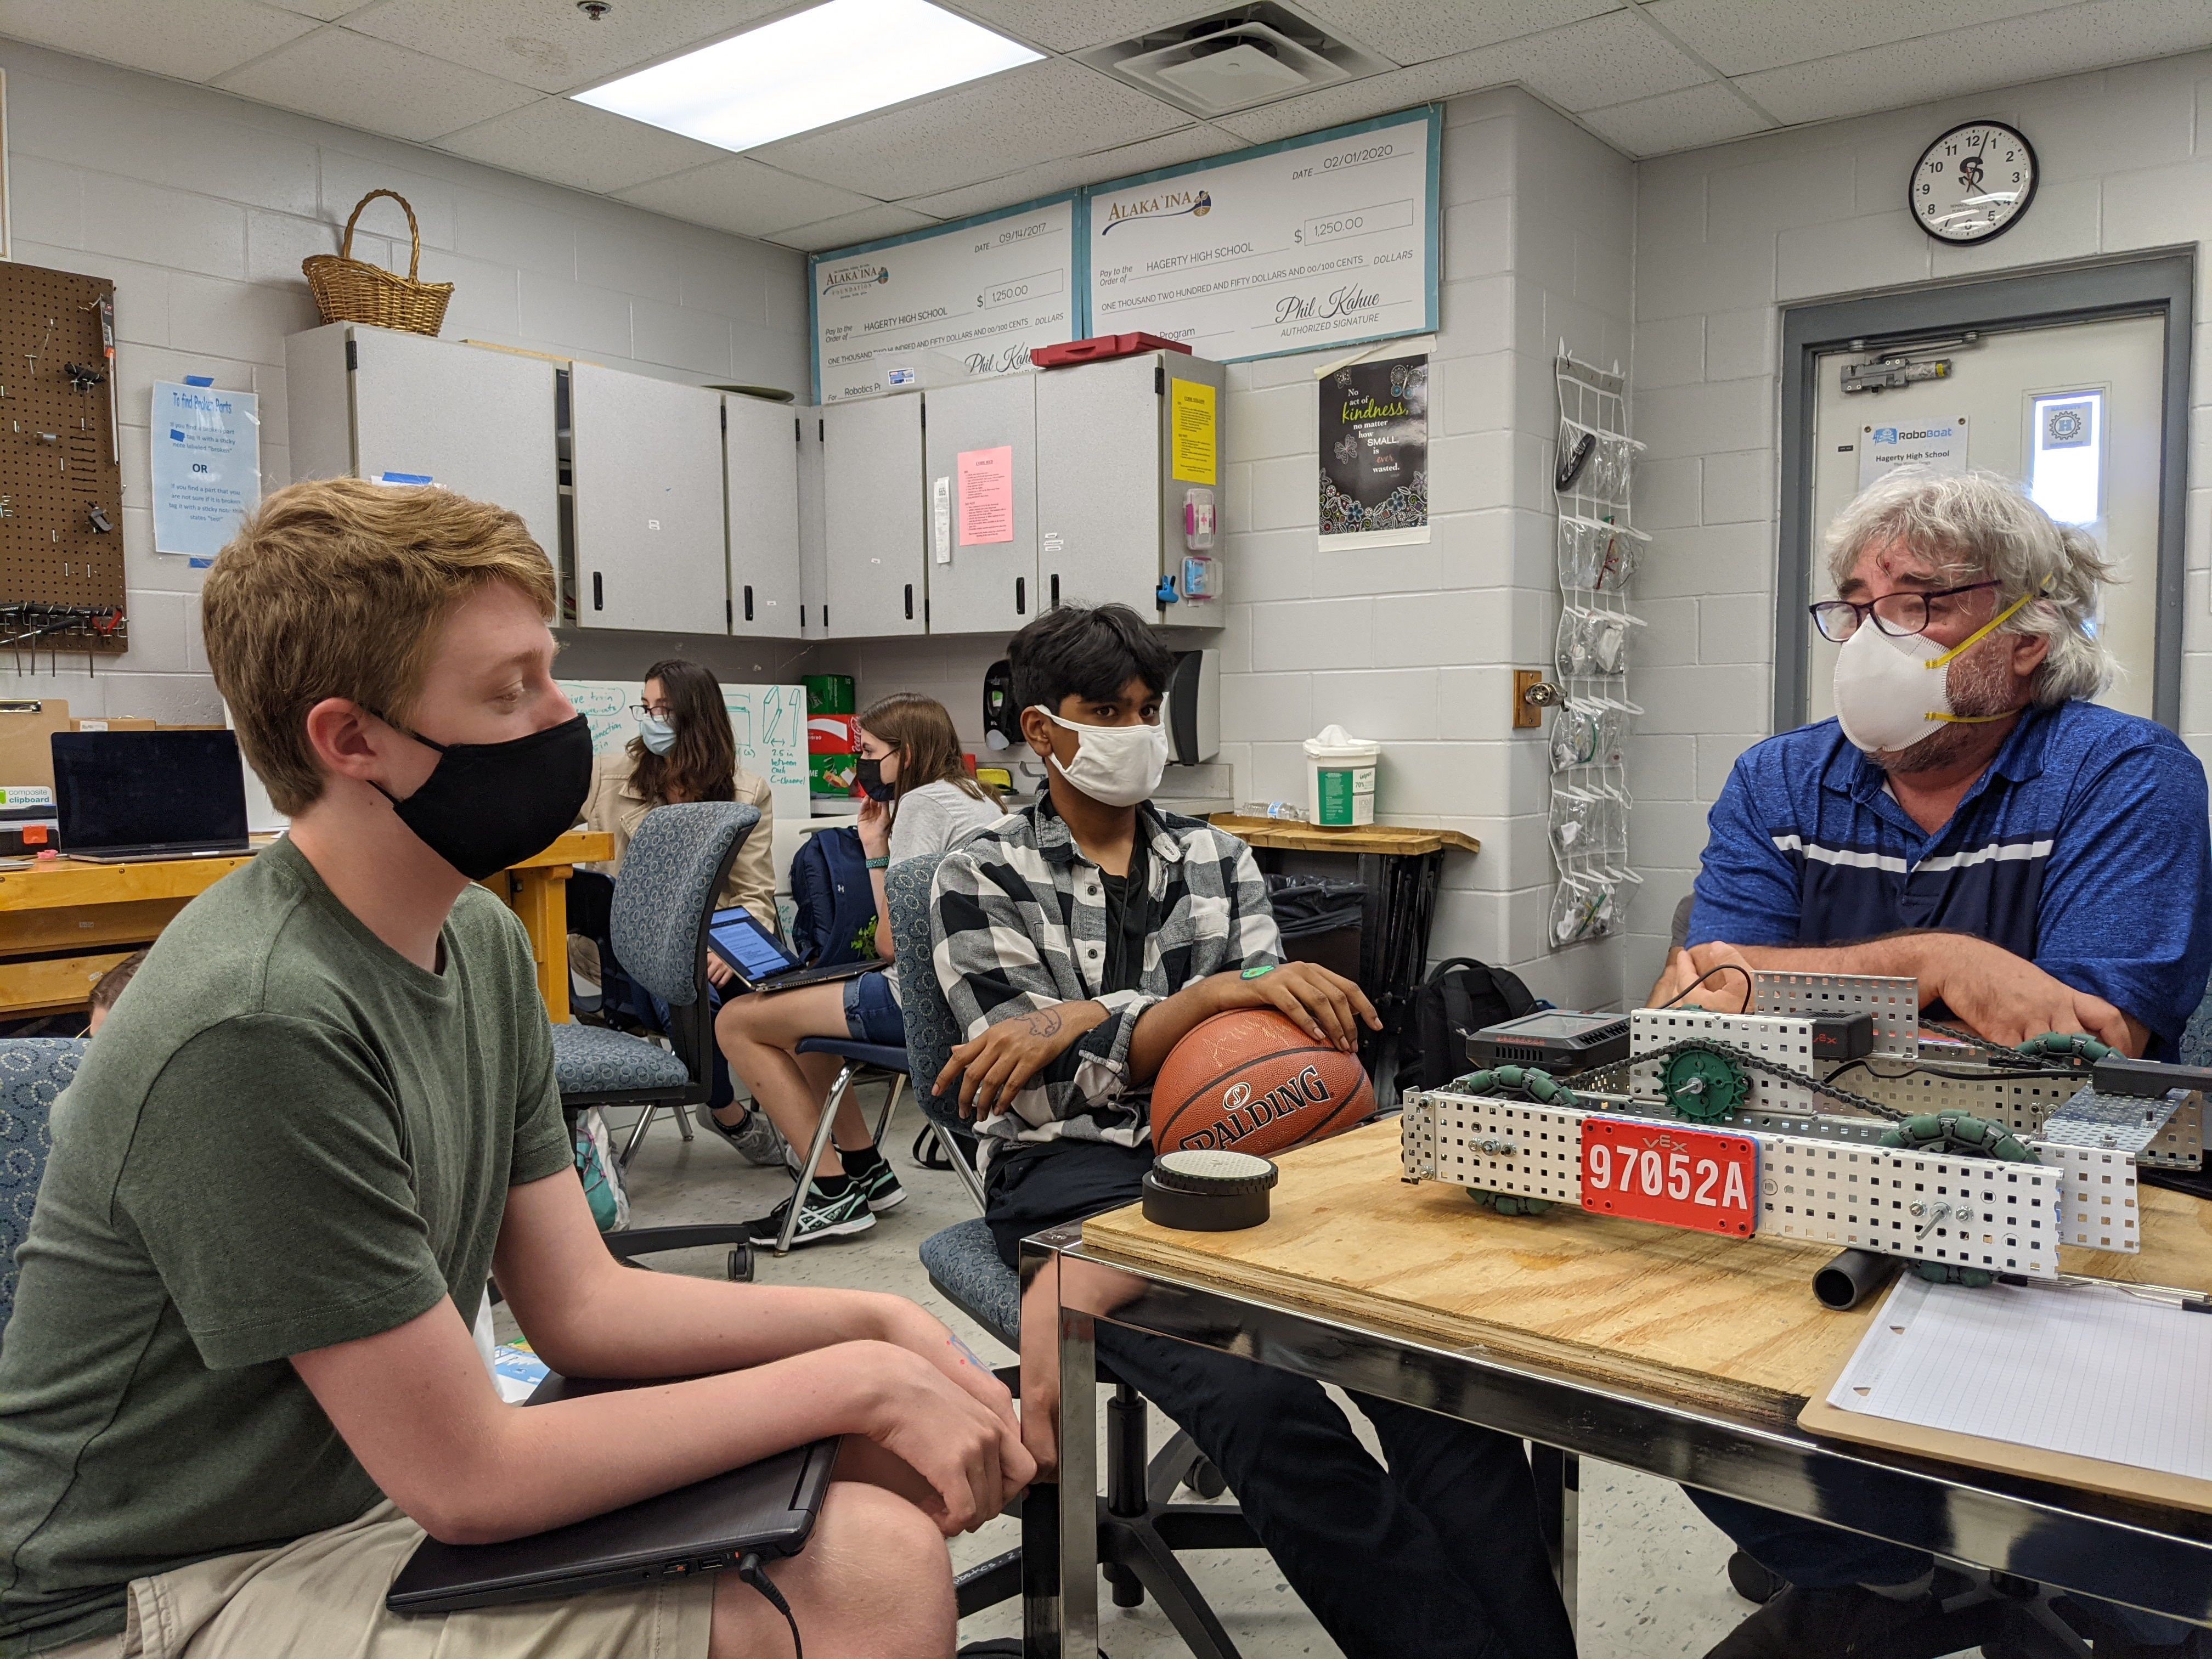
\includegraphics[width=0.9\textwidth, angle=0]{Meetings/September/09-21-21/09-21-21 1.jpg}
\caption{Discussion with Mr. Harper, our technical mentor, about solving drivetrain issues.}
\label{fig:092122_1}
\end{figure}

\hhscommittee{Multimedia}
\noindent\hfil\rule{\textwidth}{.4pt}\hfil
\subsubsection*{Goals}
\begin{itemize}
    \item Our goal for today was to read the FTC Game Manual and understand what our Promote Video theme would be for this season.  

\end{itemize} 

\noindent\hfil\rule{\textwidth}{.4pt}\hfil

\subsubsection*{Accomplishments}
We began by reading through Game Manual 1, in which we found the guidelines for the Promote Award. We noted down the requirements and uploaded a screenshot to the Google Drive. From there, we started doing some rough brainstorming, with ideas like letters to yourself or interviewing our FLL teams, and more abstract ideas like a time capsule which would incorporate the characters that we used in the animation from last season. We are considering making another animation, since it did so well last season and as a team, we enjoyed creating it and overcoming the challenges of that year. 
On another note: At the beginning of the meeting we signed the basketball that we had played with over the weekend during our team bonding event. We took photos for a social media post to announce that we had held that event and we plan on holding another game this upcoming Friday.

\begin{figure}[ht]
\centering
\begin{minipage}[b]{.48\textwidth}
  \centering
  
\includegraphics[width=0.95\textwidth]{Meetings/September/09-21-21/9-18-21_Team_Image1 - Nathan Forrer.jpg}
  \caption{The cover page for Game Manual 1.}
  \label{fig:092122_1}
\end{minipage}%
\hfill%
\begin{minipage}[b]{.48\textwidth}
  \centering
  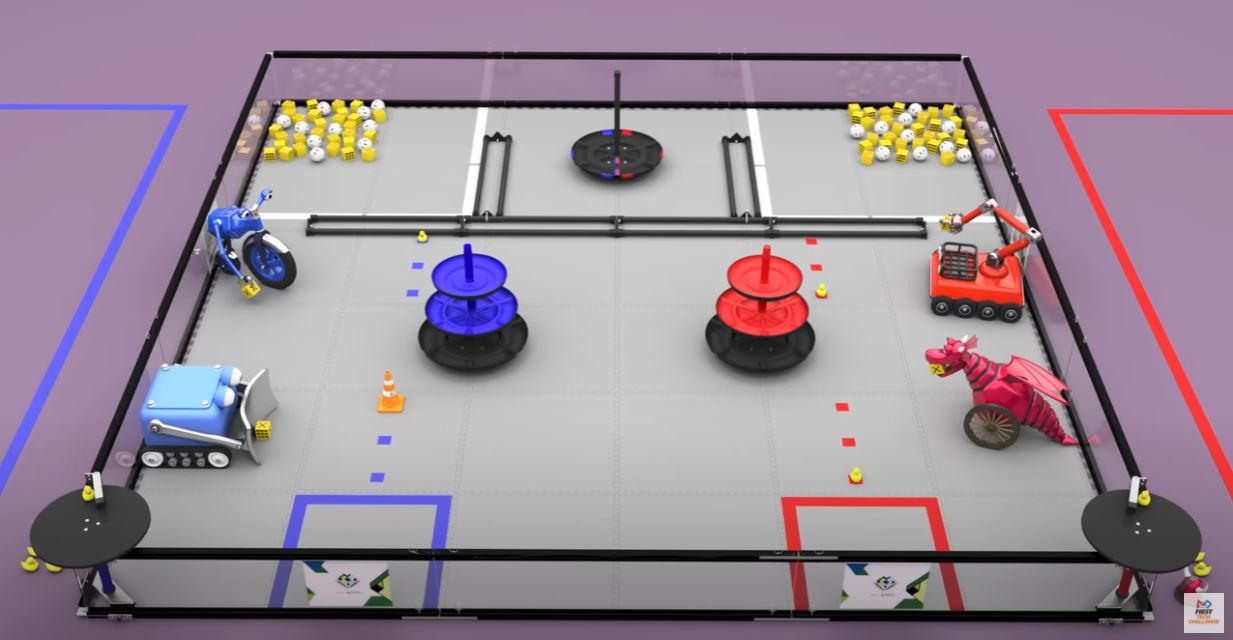
\includegraphics[width=0.95\textwidth]{Meetings/September/09-21-21/9-18-21_Team_Image2 - Nathan Forrer.jpg}
  \caption{This year's field.}
  \label{fig:092122_2}
\end{minipage}
\end{figure}

\begin{figure}[ht]
\centering
\begin{minipage}[b]{.48\textwidth}
  \centering
  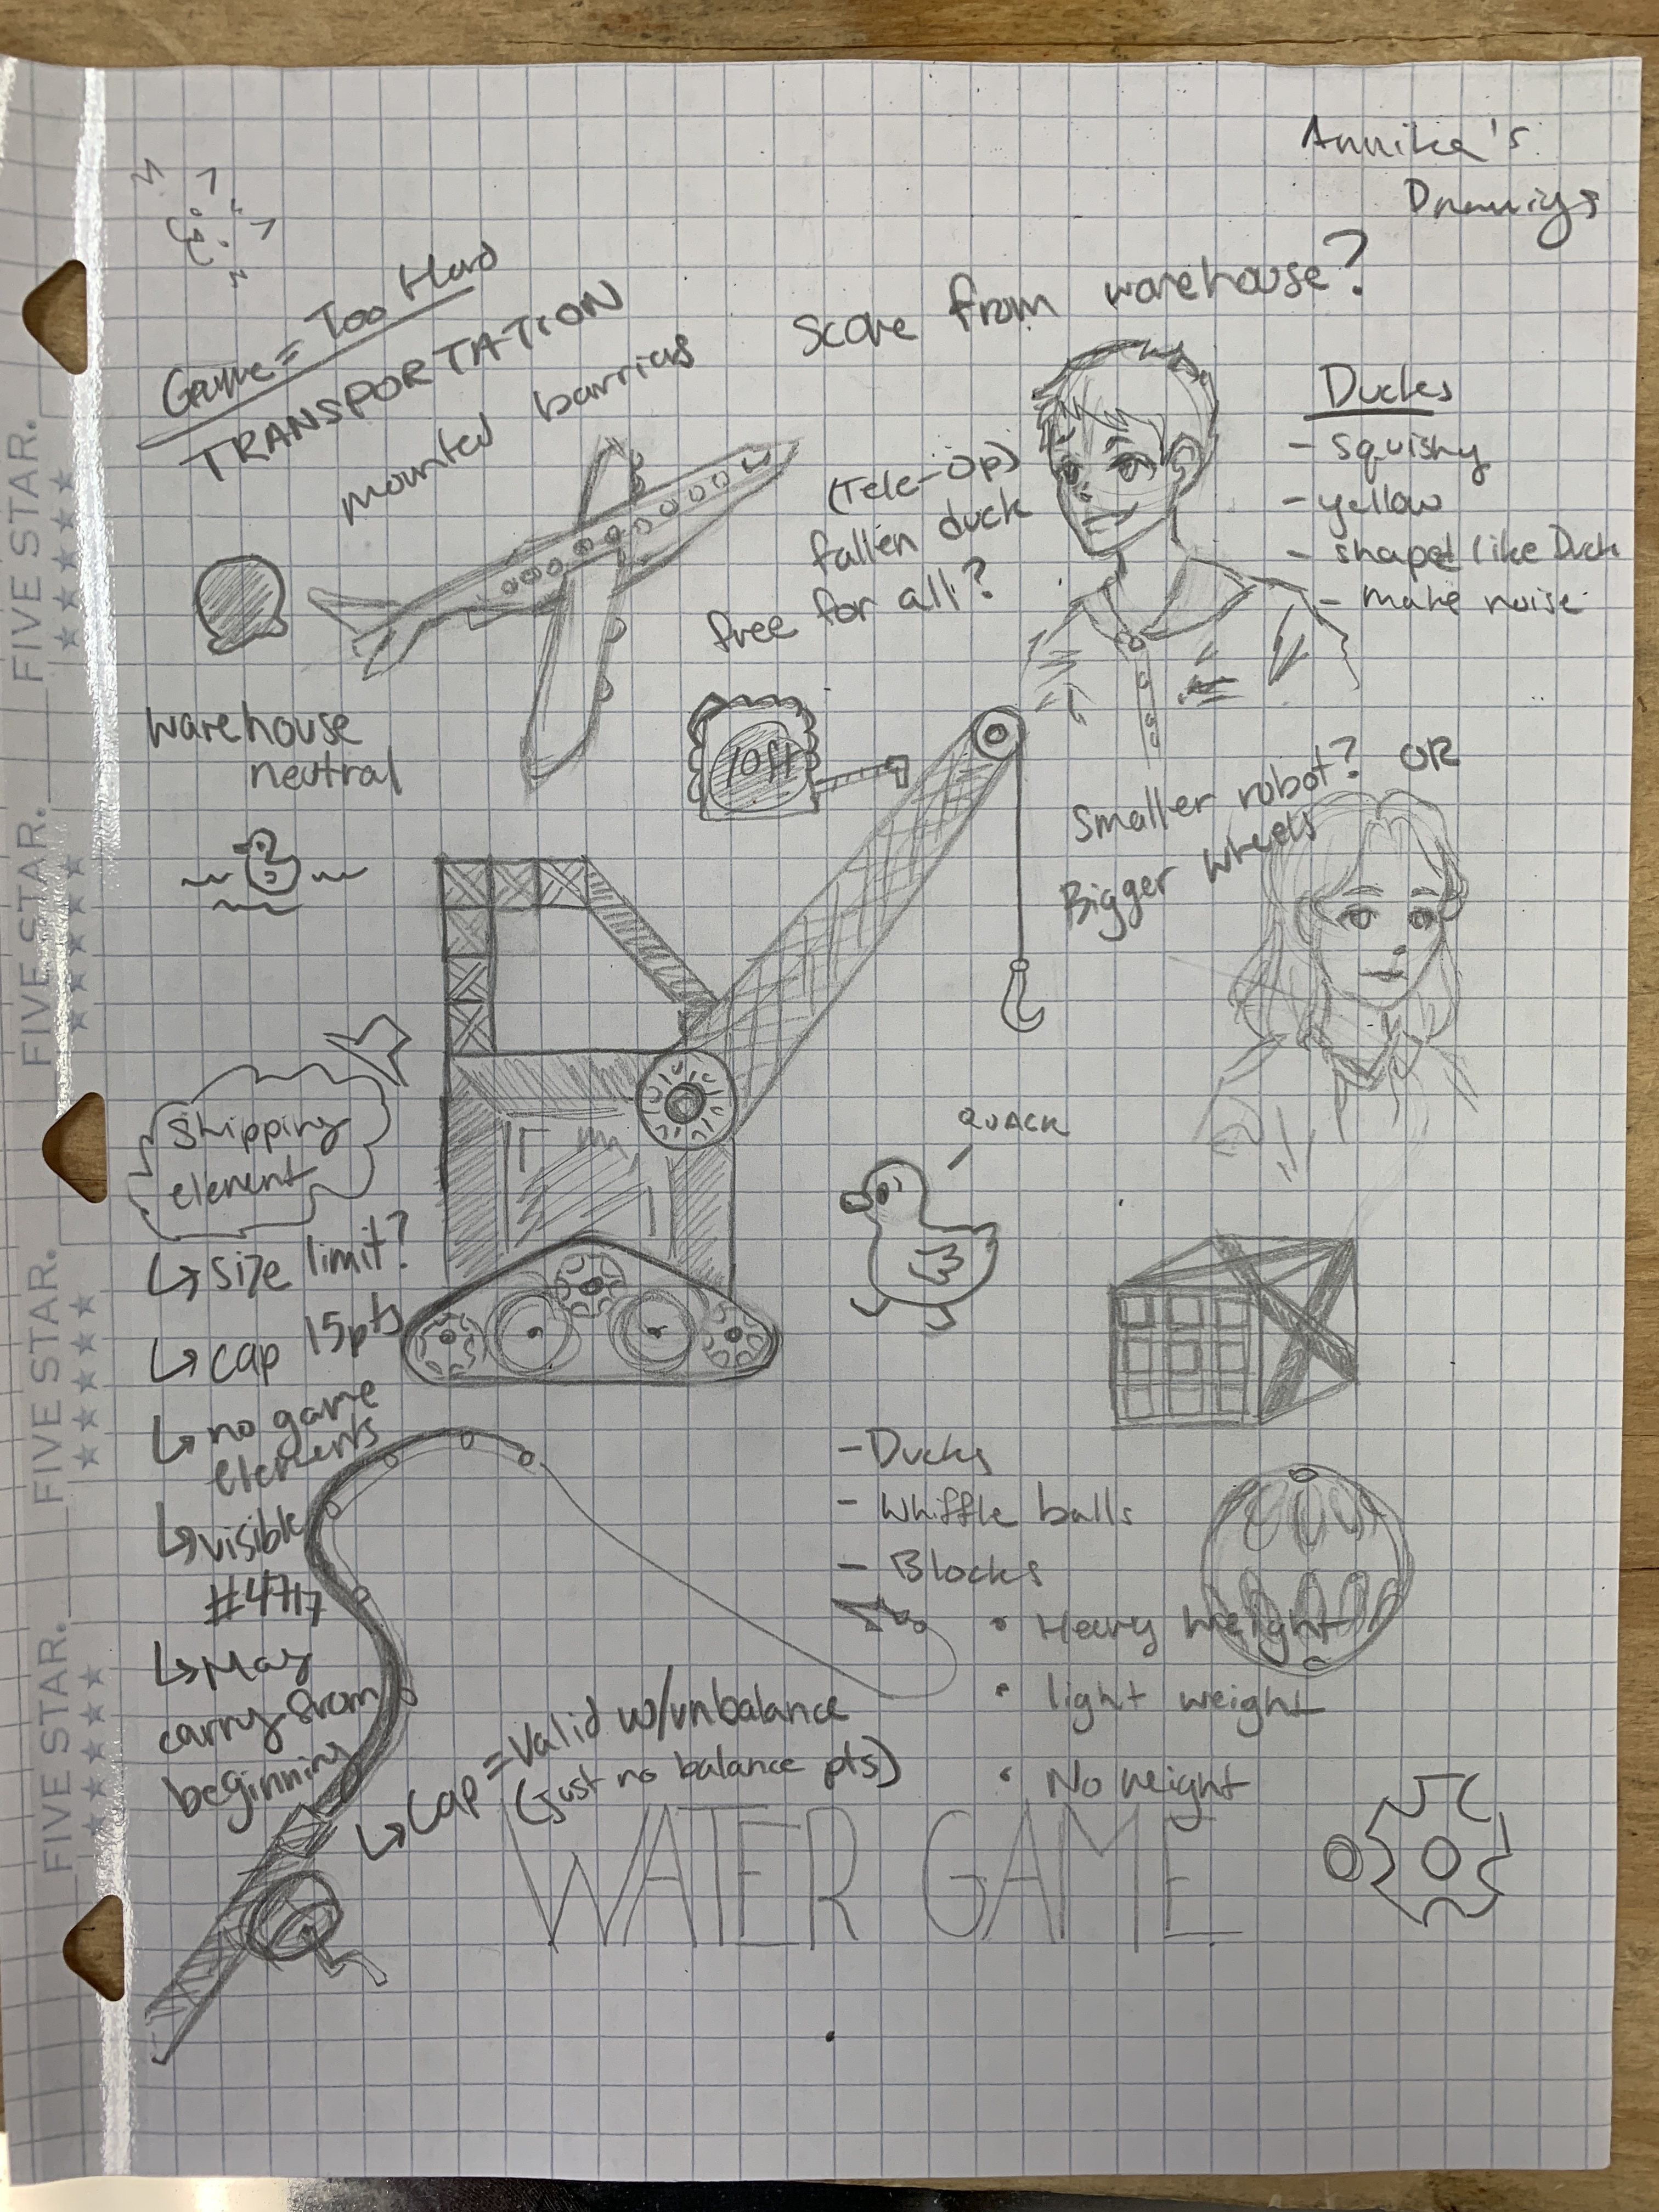
\includegraphics[width=0.95\textwidth]{Meetings/September/09-21-21/9-19-21_Team_Image3 - Nathan Forrer.JPG}
  \caption{A robot doodle page (With some bonus drawings).}
  \label{fig:092122_3}
\end{minipage}%
\hfill%
\begin{minipage}[b]{.48\textwidth}
  \centering
  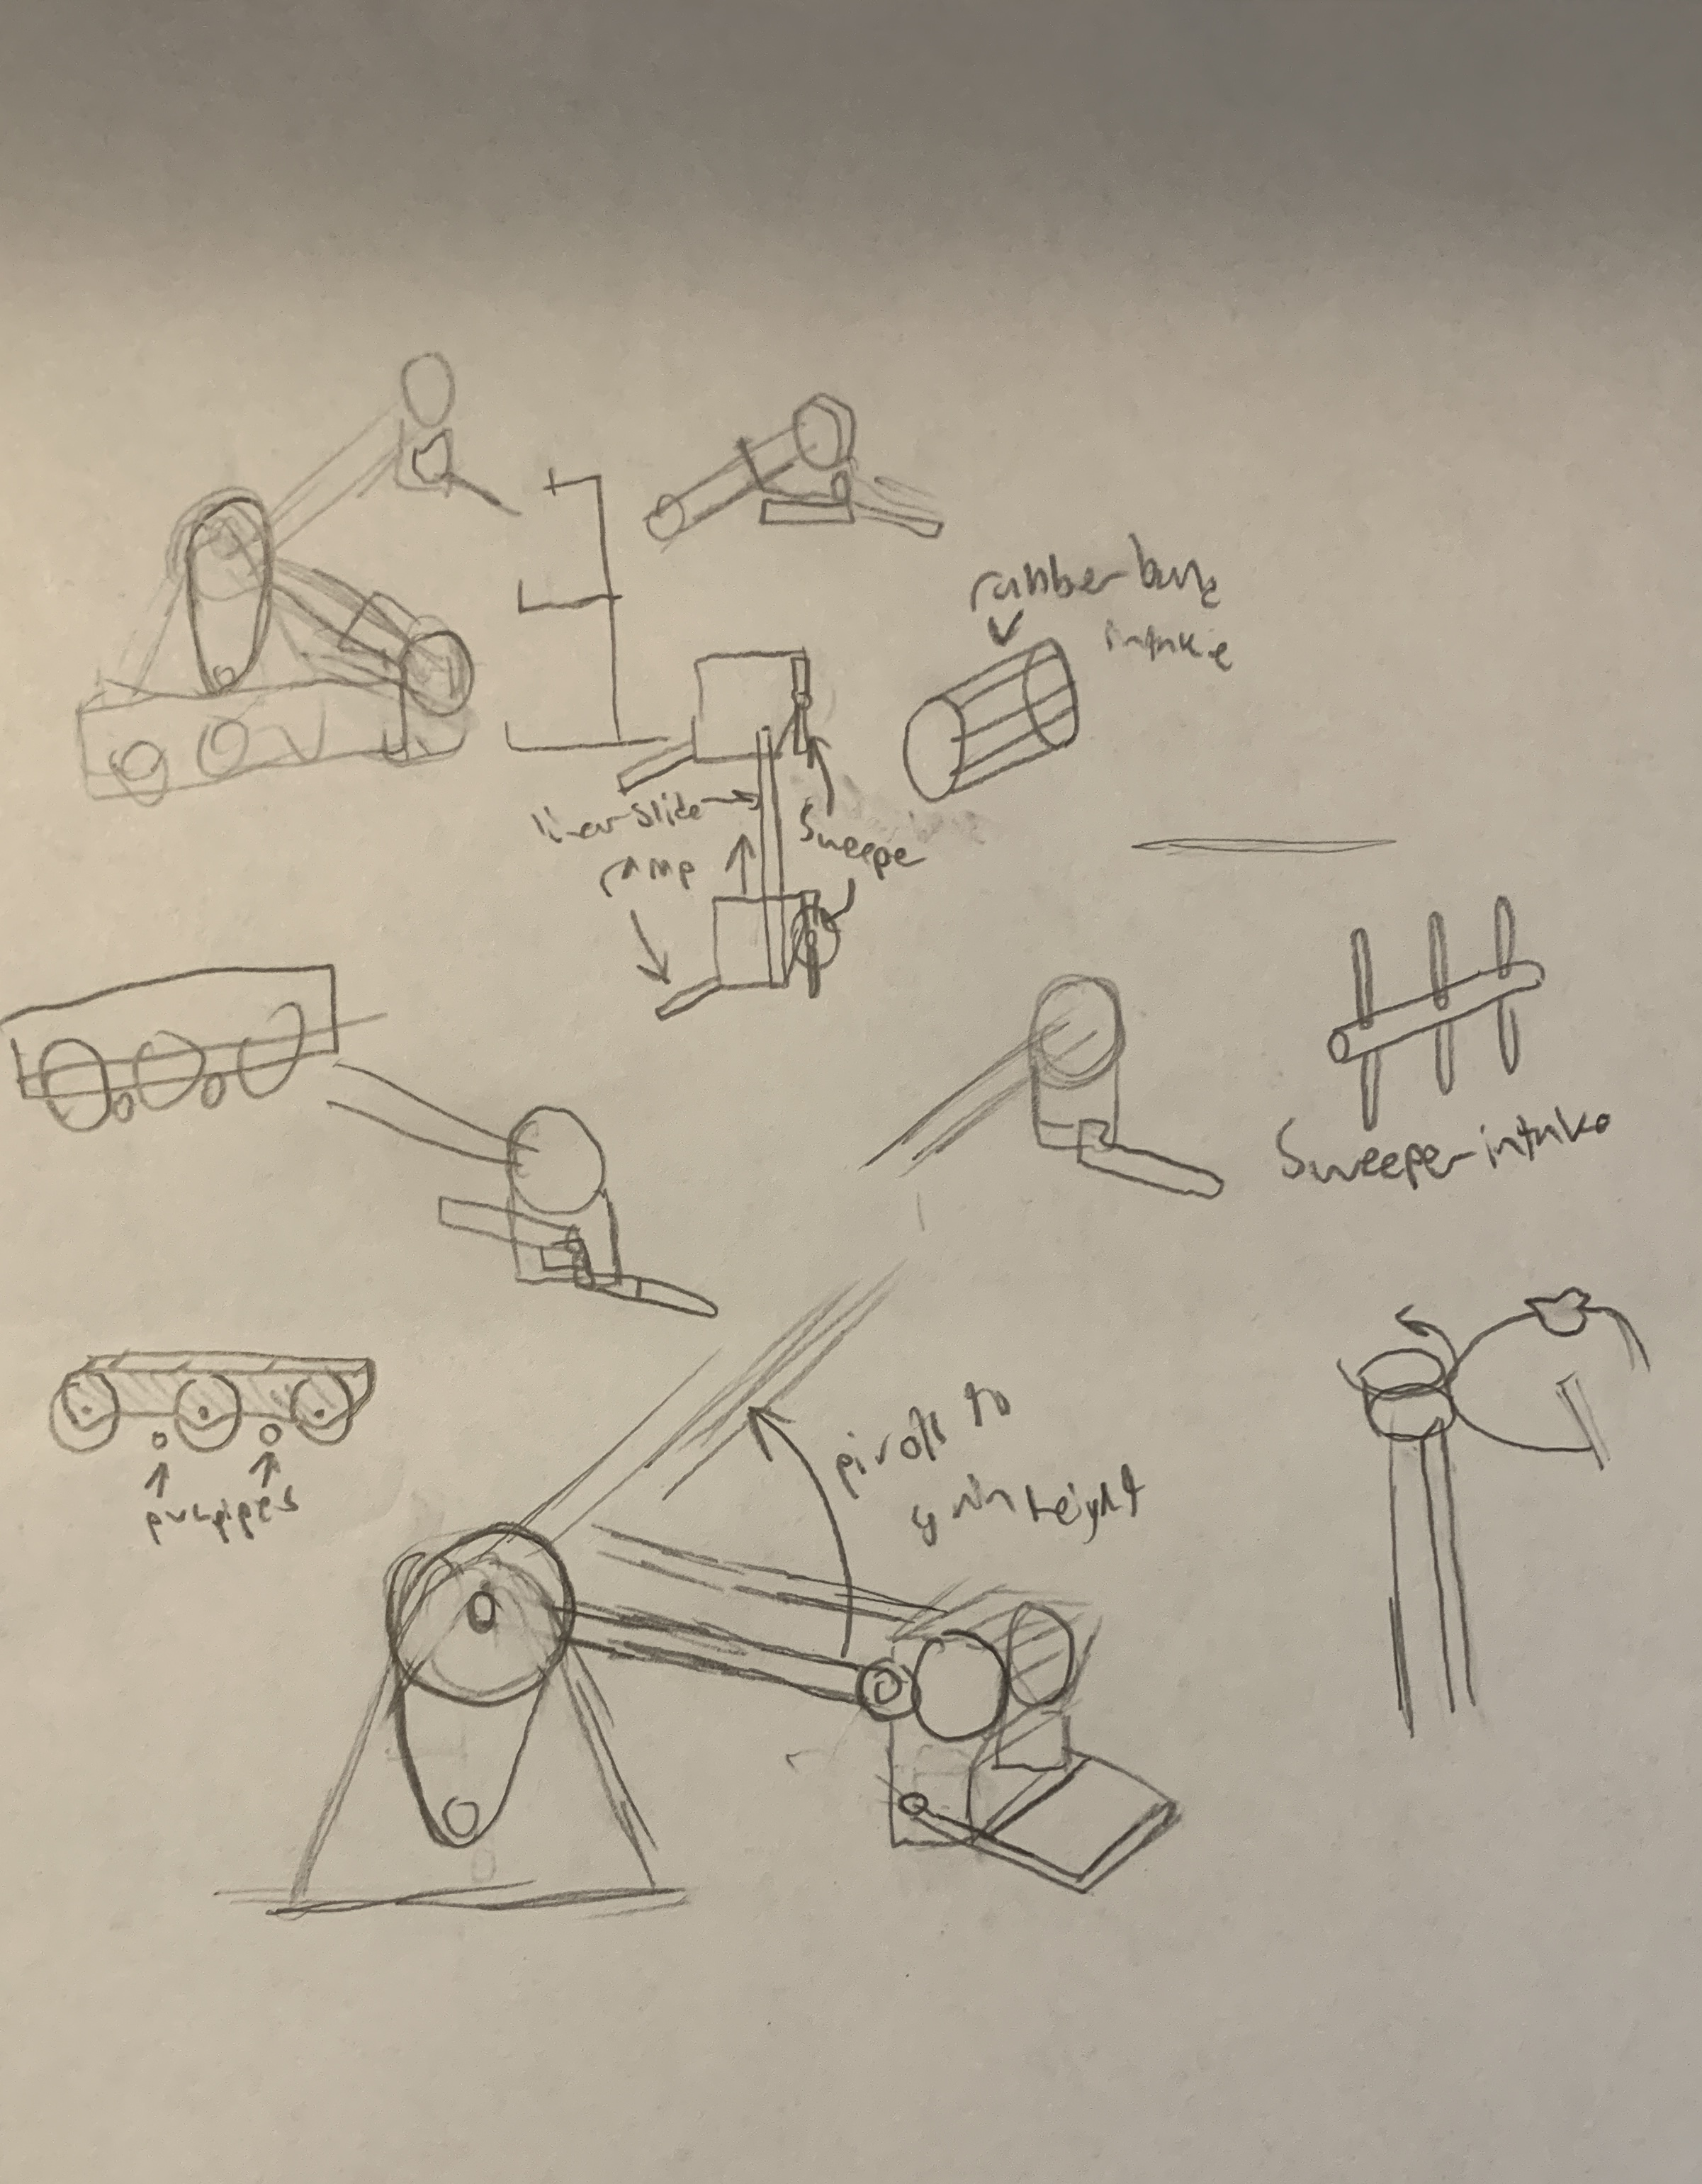
\includegraphics[width=0.95\textwidth]{Meetings/September/09-21-21/9-19-21_Team_Image4 - Nathan Forrer.JPG}
  \caption{Another page of our team's planning sketches.}
  \label{fig:092122_4}
\end{minipage}
\end{figure}

\begin{figure}[ht]
\centering
\begin{minipage}[b]{.48\textwidth}
  \centering
  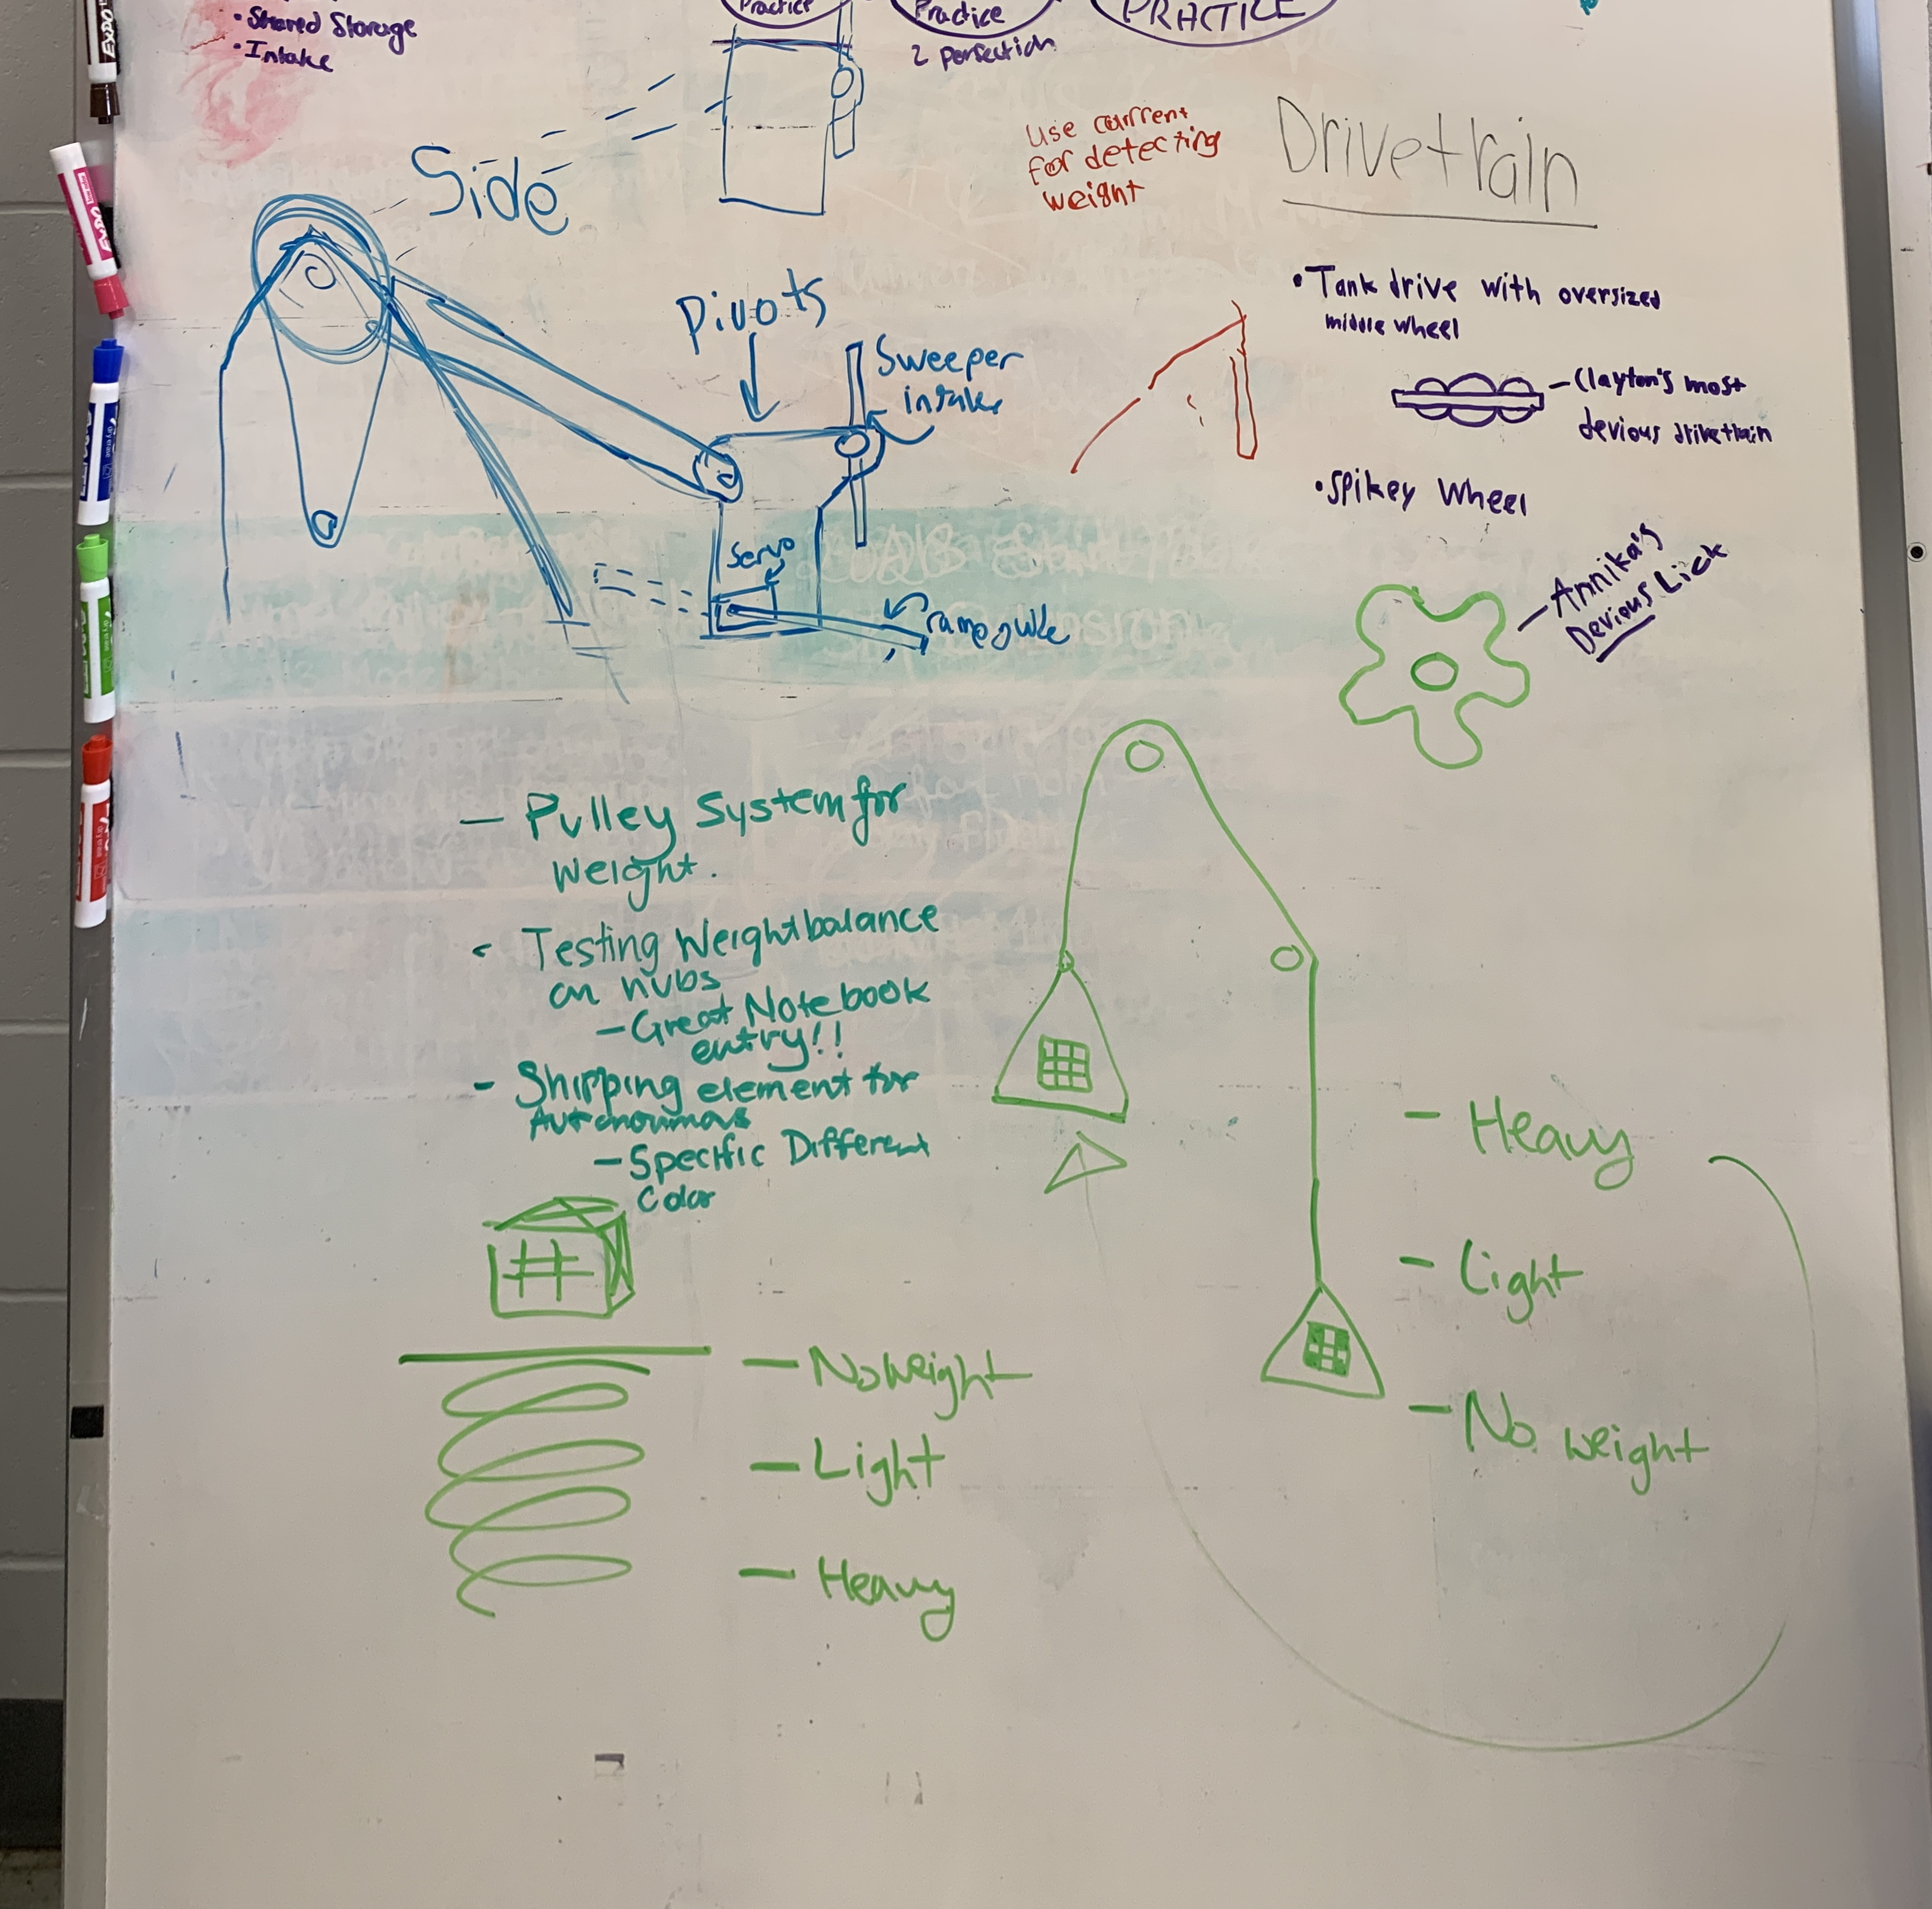
\includegraphics[width=0.95\textwidth]{Meetings/September/09-21-21/9-19-21_Team_Image5 - Nathan Forrer.JPG}
  \caption{A whiteboard with even more of our team's planning.}
  \label{fig:092122_5}
\end{minipage}%
\hfill%
\begin{minipage}[b]{.48\textwidth}
  \centering
  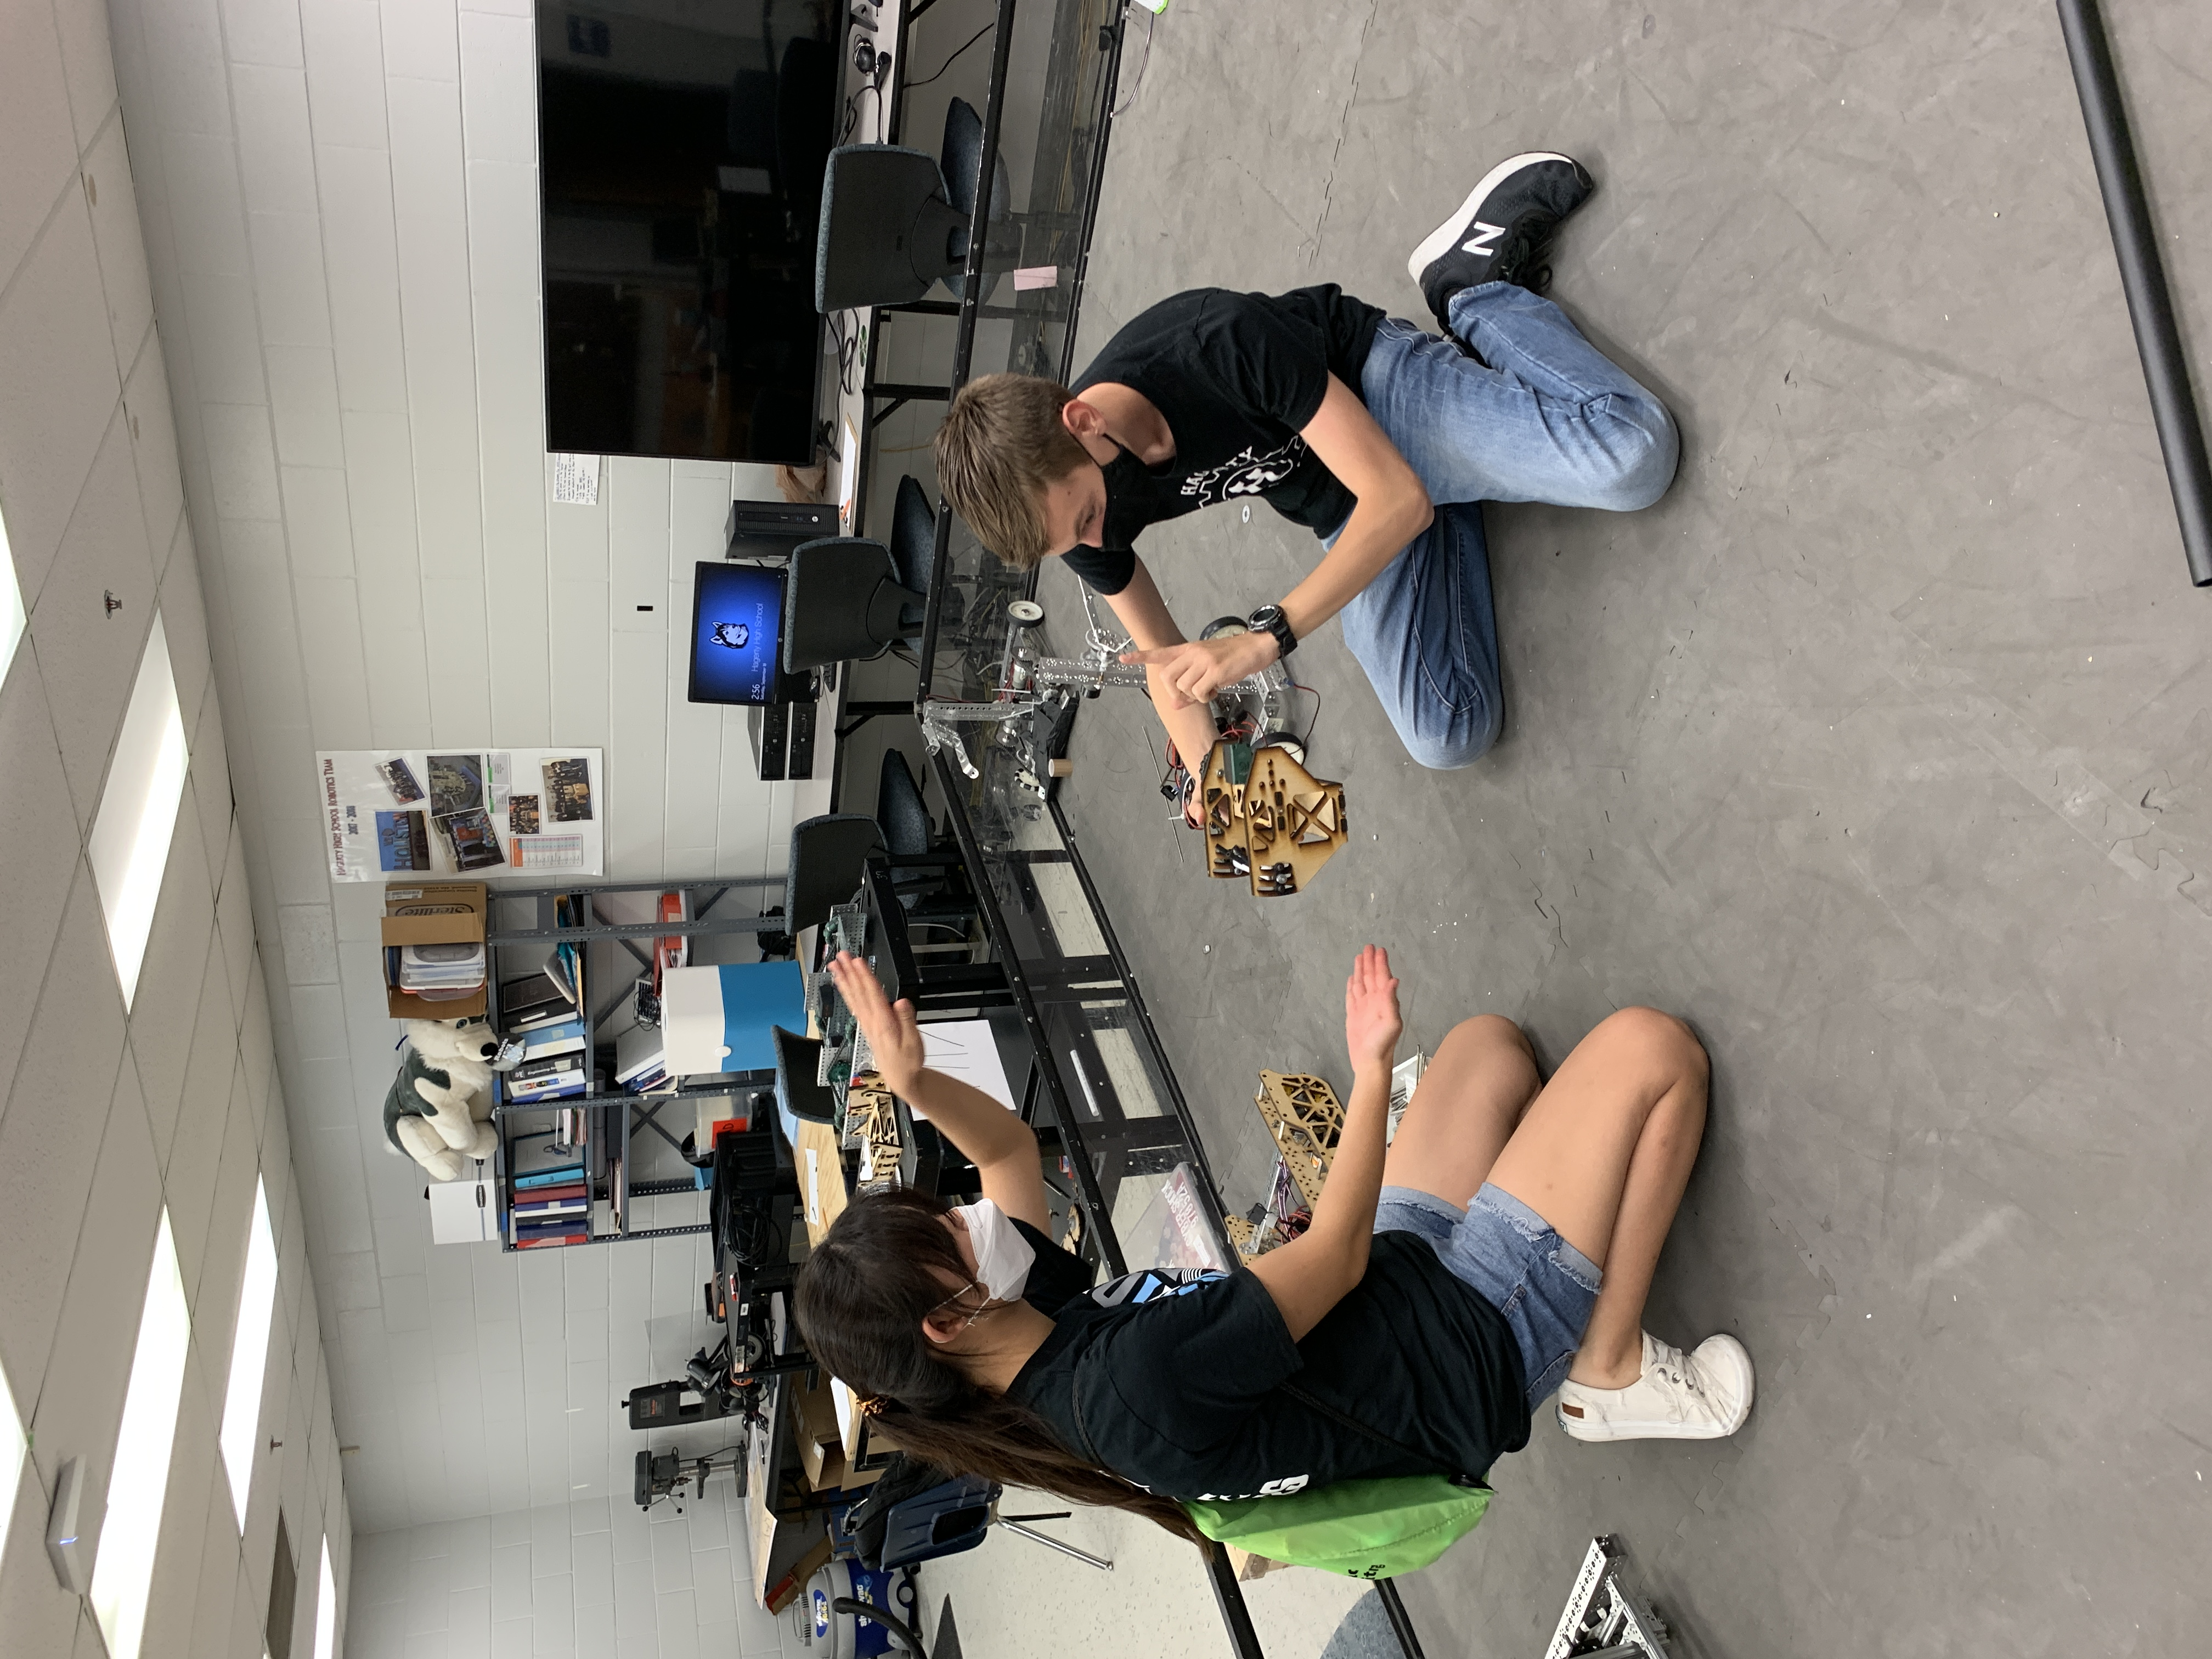
\includegraphics[width=0.95\textwidth]{Meetings/September/09-21-21/9-19-21_Team_Image6 - Nathan Forrer.JPG}
  \caption{Jensen and Annika prototyping designs.}
  \label{fig:092122_6}
\end{minipage}
\end{figure}

\begin{figure}[htp]
\centering
  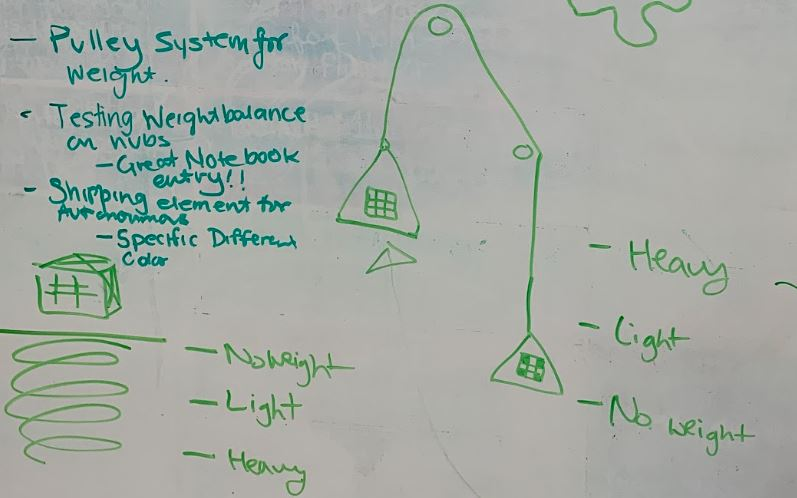
\includegraphics[width=0.95\textwidth]{Meetings/September/09-21-21/9-18-21_Team_Image7 - Nathan Forrer.jpg}
  \caption{A closeup shot of our brainstorms on a pulley system.}
  \label{fig:092122_7}
\end{figure}

\begin{figure}[htp]
\centering
  \centering
  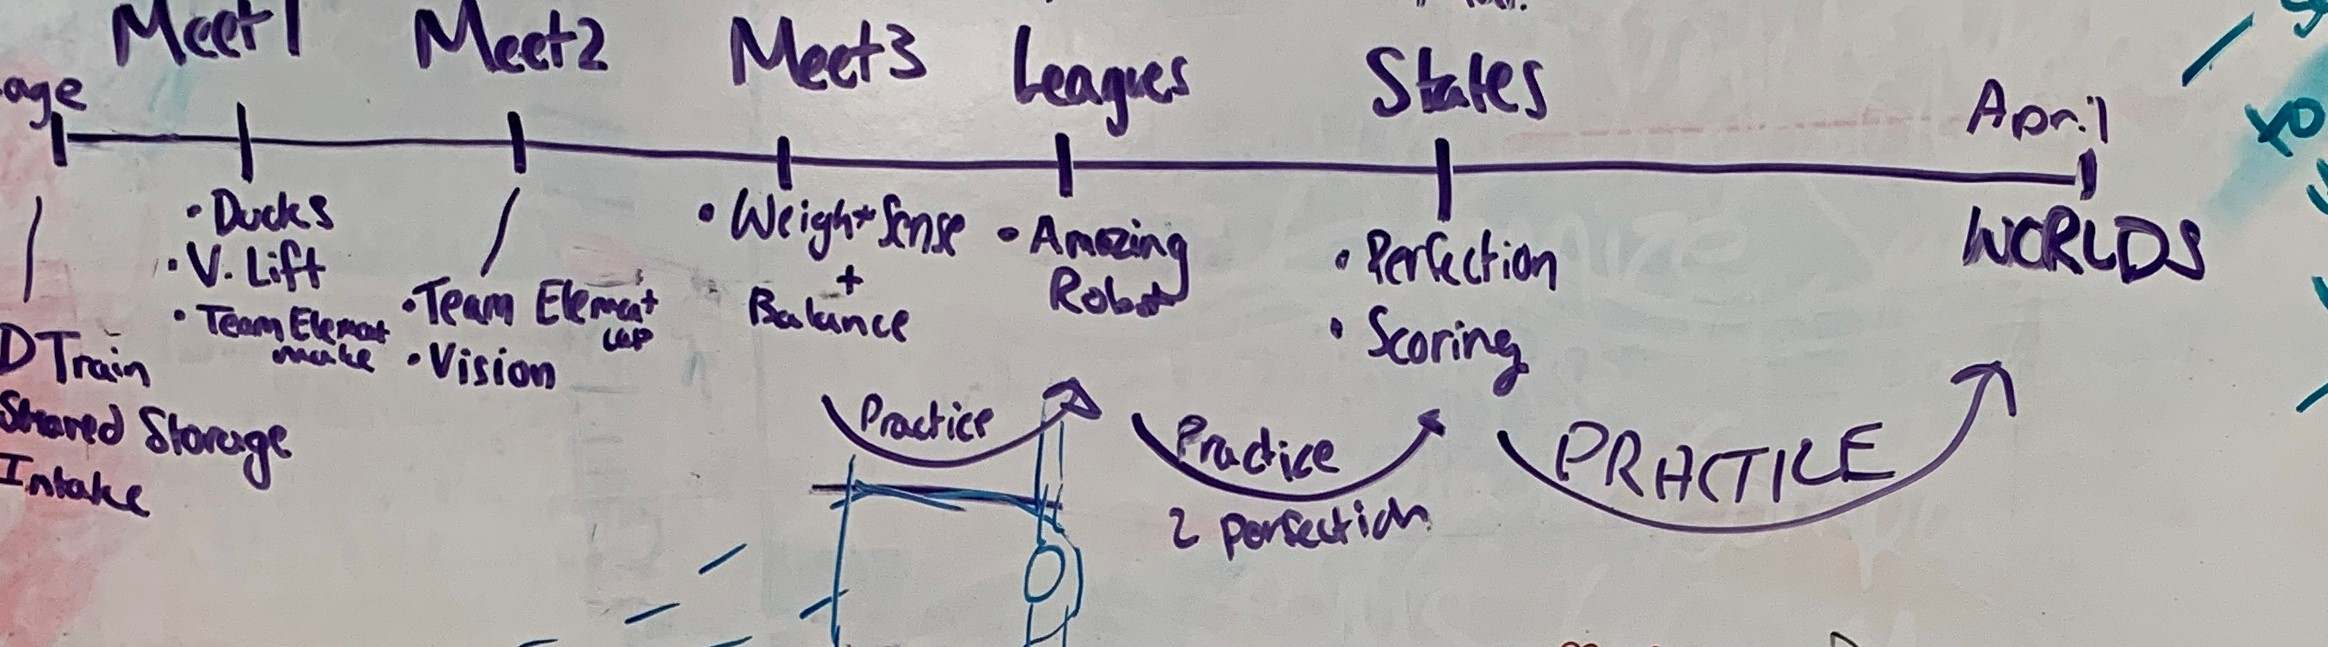
\includegraphics[width=0.95\textwidth]{Meetings/September/09-21-21/9-18-21_Team_Image8 - Nathan Forrer.jpg}
  \caption{Our timeline for this year.}
  \label{fig:092122_8}
\end{figure}

\whatsnext{
\begin{itemize}
    \item Build and fully decide on intake.
    \item Next meeting, we plan to do more brainstorming and think of ways to incorporate the FIRST Core Values and Gracious Professionalism into the video.
\end{itemize} 
}
